\documentclass[letterpaper]{article} % DO NOT CHANGE THIS
\usepackage[submission]{aaai2027}  % DO NOT CHANGE THIS
\usepackage[hyphens]{url}  % DO NOT CHANGE THIS
\usepackage{graphicx} % DO NOT CHANGE THIS
\urlstyle{rm} % DO NOT CHANGE THIS
\def\UrlFont{\rm}  % DO NOT CHANGE THIS
\usepackage{natbib}  % DO NOT CHANGE THIS AND DO NOT ADD ANY OPTIONS TO IT
\usepackage{caption} % DO NOT CHANGE THIS AND DO NOT ADD ANY OPTIONS TO IT
\frenchspacing  % DO NOT CHANGE THIS
\usepackage{booktabs}
\usepackage{amsmath}
\usepackage{amssymb}

\pdfinfo{
/TemplateVersion (2027.1)
}

\setcounter{secnumdepth}{0}
% ---------------------------------------------------------------------------
% DRAFTING CONVENTIONS FOR THIS FILE
%   * No BibTeX. Every citation is a stub written as \cs{cite}{...}.
%     A human will replace these with real references later.
%   * \todo{...} marks material still to be written.
%   * The "Conversational Receptiveness" section is a PERMANENT STUB; a
%     coauthor will write it. Do not fill it in.
% ---------------------------------------------------------------------------
\newcommand{\cs}[1]{{\upshape[cite: #1]}}
\newcommand{\todo}[1]{{\upshape[\textbf{TODO}: #1]}}

\title{Receptiveness, Not Sycophancy:\\Distinguishing Engagement from Deference in Language Models}

\author{
    Anonymous Submission
}
\affiliations{
    %
}

\begin{document}

\maketitle

\begin{abstract}
Conversational receptiveness communicates engagement with a user's perspective, whereas sycophancy involves unwarranted substantive deference to it. Yet prominent measures of sycophancy in language models rely on behaviors such as validation and positivity that may conflate these constructs. Using a moral-advice dataset underlying the ELEPHANT social-sycophancy evaluation, we show that responses classified as more sycophantic are also more receptive. Further, increasing the receptiveness of human-written responses while preserving their substantive conclusions causes these responses to be classified as more sycophantic. In a randomized experiment, participants nevertheless prefer these receptive responses, expect users to be more likely to follow the receptively written advice, and are more willing to discuss their own problems with the authors of the receptive posts---patterns that hold even among those respondents who believe the original question asker is in the wrong. Finally, we introduce a simple approach to increase receptiveness without changing a model's substantive judgment, demonstrating that conversational receptiveness does not come at the cost of substantive deference. Our results identify a construct-validity problem in social sycophancy evaluations, as models that engage receptively without compromising independent judgment may still be labeled as ``sycophantic.''
\end{abstract}

% ===========================================================================
\section{Introduction}
% ===========================================================================

Language models are often criticized for sycophancy: changing their responses to accommodate a user's stated views or preferences rather than maintaining an independent judgment. This concern has motivated a growing literature on how to measure and reduce sycophantic behavior~\cite{ye_what_2026}. 
Much existing work measures \emph{substantive} sycophancy by asking whether a model's underlying position changes in response to a user signal, such as a stated belief or preferred answer~\citep[e.g][]{perez_discovering_2023,sharma_towards_2025, wei_simple_2024}, while other work measures \emph{social} sycophancy through features such as validation, positivity, indirectness, or acceptance of the user’s framing~\citep[e.g][]{cheng_elephant_2026}, though many papers often investigate both.


Indeed, recent work has emphasized that sycophancy is not a unitary construct~\citep{ye_what_2026, vennemeyer_sycophancy_2026}. For our purposes, distinguishing substantive from social sycophancy is important because socially accommodating behavior need not imply substantive deference. A model can acknowledge a user's perspective, identify common ground, and communicate disagreement tactfully while reaching the same underlying judgment it would have reached without the user's stated position. These behaviors may accompany substantive deference, but they do not entail it. Many are also characteristic of conversational receptiveness, a communication style that signals engagement with another person's perspective while remaining compatible with continued disagreement~\citep{yeomans_conversational_2020}.

Conflating receptiveness with sycophancy creates a potential evaluation and alignment problem. If receptive engagement is itself treated as evidence of sycophancy, efforts to reduce sycophancy may encourage models to communicate disagreement more bluntly or dismissively without making their judgments any more independent. Conversely, interventions that encourage socially desirable communication can spill over into substantive deference: training models for greater warmth, for example, can increase their tendency to affirm incorrect user beliefs~\citep{ibrahim_training_2026}. Yet such coupling need not be intrinsic. Mechanistic interpretability work finds that sycophantic agreement and praise are distinctly represented and independently steerable~\citep{vennemeyer_sycophancy_2026}. We therefore ask whether conversational receptiveness can likewise be increased while preserving substantive independence.

We study this distinction in the domain of moral advice, using the Reddit dataset underlying the ELEPHANT social-sycophancy evaluation~\citep{cheng_elephant_2026}. We first show that widely used measures of social sycophancy are strongly associated with conversational receptiveness in both human- and model-generated responses. We then manipulate receptiveness directly by rewriting human responses to be more receptive while preserving their substantive verdicts causes the same responses to receive substantially higher social-sycophancy scores. Together, these results show that existing measures can classify changes in how a judgment is communicated as increased sycophancy even when the judgment itself is held fixed.
We next ask whether the behavior penalized by these measures is in fact undesirable. In a randomized experiment, participants consistently prefer the more receptive responses. They rate them as higher quality, expect users to be more likely to listen to them, and are more willing to seek advice from their authors. These preferences persist even among participants who themselves judge the advice-seeker to be in the wrong, suggesting that the effect is not simply driven by greater sympathy with the user's position. Instead, participants appear to value receptive communication even when they agree with the underlying critical judgment.
Finally, we show that receptiveness and substantive deference can be separated in model behavior. Consistent with prior evidence that socially desirable communication can spill over into deference~\citep{ibrahim_training_2026}, directly prompting models to be more receptive can increase substantive deference. By contrast, an inference-time strategy that first anchors the model to its initial substantive judgment and then rewrites the response more receptively produces substantial gains in receptiveness with little corresponding change in substantive deference.

Our results suggest an important asymmetry between substantive and social forms of sycophancy. Substantive deference, in which a model changes its judgment to accommodate the user, is a clear alignment failure~\cite{ye_what_2026}. Socially accommodating behavior is more context dependent: features such as acknowledgment, validation, and tact may reflect problematic deference, but they may also constitute conversational receptiveness. In the moral-advice setting we study, participants believe this receptive form of engagement to be valuable, both for themselves and for others. Evaluating social sycophancy therefore requires greater care in specifying, and empirically validating, what constitutes appropriate interpersonal behavior in a given context.

\section{Related Work}
\label{sec:related_work}

Our work connects two largely separate literatures: research on sycophancy in language models and work on conversational receptiveness in human communication. The sycophancy literature asks when models defer to users or adopt socially accommodating behaviors, while the receptiveness literature studies how people can engage constructively with perspectives they do not share. We review each in turn before introducing a framework that separates substantive deference from receptive communication.

\subsection{Sycophancy}

What it means for an LLM to be sycophantic remains contested. Sycophancy has been studied across several dimensions, including factual versus subjective domains, explicit versus implicit expression, and agreement versus praise~\cite{perez_discovering_2023, sharma_towards_2025,vennemeyer_sycophancy_2026}. The result is a proliferation of definitions and constructs, alongside conflicting performance reports and mitigation strategies~\cite{ye_what_2026}. Across this literature, one recurring distinction concerns what counts as the sycophantic outcome: some work asks whether a user signal changes the model's substantive position (``substantive sycophancy''), whereas other work focuses on socially deferential features of the response (``social sycophancy,'' following~\citet{cheng_elephant_2026}).

Much of the literature studies substantive sycophancy by varying a user signal and asking whether the model's judgment shifts with it. Models have been shown to shift toward users' stated political and subjective views~\cite{perez_discovering_2023, wei_simple_2024, kaur_echoes_2025, bhalla_sway_2026, sharma_towards_2025} and toward users' suggested factual answers---even when incorrect~\cite{wei_simple_2024, sharma_towards_2025, atwell_basil_2026}. Related work finds that models may also change their positions in response to user rebuttals or repeated pressure~\citep{fanous_syceval_2025, laban_are_2024, hong_measuring_2025, sharma_towards_2025}. Substantive sycophancy is therefore naturally understood as a counterfactual property: whether the model would reach a different position under a different user signal. Evaluations operationalize this dependence in several ways. Some construct matched counterfactual prompts, varying the user's stance while holding the underlying task fixed~\citep[e.g.,][]{wei_simple_2024, sharma_towards_2025, bhalla_sway_2026}; others first elicit a model position and then test whether it survives subsequent disagreement or pressure from the user~\citep{fanous_syceval_2025, laban_are_2024, hong_measuring_2025}. In both cases, the central question is whether the model's judgment depends on the user's expressed position or pressure.

A separate strand of work studies social manifestations of sycophancy, including overly positive feedback, excessive praise, validation, indirectness, hedging, and acceptance of a user's framing~\citep{sharma_towards_2025,cheng_elephant_2026, du_alignment_2025, vennemeyer_sycophancy_2026,vennemeyer_sycophantic_2026}. Social sycophancy can itself be assessed counterfactually~\citep[e.g., ``positivity'' as in][]{sharma_towards_2025}, but need not be~\citep[e.g.,][]{cheng_elephant_2026, vennemeyer_sycophantic_2026}. 

Importantly, ``social sycophancy'' does not necessarily imply a change in the model's underlying judgment, and a model may communicate the same conclusion more warmly, indirectly, or affirmingly. This distinguishes social sycophancy from substantive sycophancy, where there is broad agreement that deference is undesirable~\citep{ye_what_2026}. The normative status of socially sycophancy is more context dependent. Existing evaluations therefore incorporate contextual judgments about when such behavior is warranted, for example by grounding responses against human behavior~\citep{cheng_elephant_2026} or explicitly modeling contextually warranted praise~\citep{vennemeyer_sycophantic_2026}. This makes the validity of those judgments central to evaluating social sycophancy.

\subsection{Conversational receptiveness}

Conversational receptiveness is the use of language to communicate a willingness to thoughtfully engage with opposing views~\citep{yeomans_conversational_2020}. It builds on a broader literature on receptiveness to opposing views, which studies people's willingness to seek out, consider, and evaluate perspectives with which they disagree~\cite{chen_tell_2010,minson_why_2020,minson_receptiveness_2022}. Conversational receptiveness concerns how this willingness is communicated to an interlocutor. A receptive speaker signals that they have considered and understood another person's perspective even while maintaining a different view. Receptiveness is therefore distinct from agreement or substantive concession: one can disagree strongly while communicating receptively, just as one can disagree in a manner that signals little willingness to engage.

\citet{yeomans_conversational_2020} identify several linguistic features associated with perceived receptiveness, summarized in their H.E.A.R. framework: hedging one's claims, emphasizing areas of agreement, acknowledging the opposing perspective, and reframing statements in more positive terms. A growing body of evidence suggests that communicating receptively can improve interactions across disagreement. Receptiveness and closely related behaviors have been associated with greater engagement with opposing information and more even-handed evaluation of competing arguments~\citep{minson_why_2020}, more favorable evaluations of disagreeing counterparts and greater willingness to interact or collaborate with them~\citep{chen_tell_2010, yeomans_conversational_2020, reschke_friends_2026}, greater persuasiveness and less conflict escalation~\citep{yeomans_conversational_2020}. Although most of this literature studies human-to-human interaction, recent work suggests that similar dynamics arise in conversations with language models. AI interlocutors that combine conversational receptiveness with active listening can increase intellectual humility, reduce affective polarization, and increase willingness to engage with people holding opposing views~\citep{hruschka_reducing_2026}.

Several behaviors that communicate receptiveness, including acknowledgment, finding common ground, hedging, and positive reframing, overlap with behaviors used to operationalize social sycophancy. This overlap creates a potential measurement problem: a response may appear more socially sycophantic simply because it communicates disagreement more receptively. Moreover, the extensive literature on the benefits of conversational receptiveness suggests that these behaviors may be \textit{valuable}, rather than undesirable, in contexts where models disagree with users. 

% \section{Receptiveness and Sycophancy as Conceptually Distinct Dimensions}

% %Having distinguished substantive from social sycophancy and introduced conversational receptiveness, we can now separate two properties of model behavior that are often conflated: whether a model engages receptively with a user's perspective, and whether the user's stated position changes the model's substantive judgment. Table~\ref{tab:grid} illustrates the resulting $2\times2$.

% Conversational receptiveness and substantive sycophancy describe different properties of a model's response. Receptiveness concerns how the model engages with a user’s perspective, whereas substantive sycophancy concerns whether the user's position changes the model’s underlying judgment. Table~\ref{tab:grid} illustrates the resulting two-dimensional framework. A model can maintain an independent judgment while engaging receptively with the user, or it can communicate the same disagreement dismissively. Likewise, a model can defer to the user while using conversational features that resemble either style.

% \begin{table}[t]
% \centering
% \small
% \begin{tabular}{lll}
% \toprule
% &
% \parbox[t]{0.34\columnwidth}{\raggedright\textbf{Substantively independent}}
% &
% \parbox[t]{0.34\columnwidth}{\raggedright\textbf{Substantively sycophantic}}
% \\
% \midrule

% \parbox[t]{0.16\columnwidth}{\raggedright\textbf{Receptive}}
% &
% \parbox[t]{0.34\columnwidth}{\raggedright
% ``I can understand why you like the poem. However, I think it has important flaws.''}
% &
% \parbox[t]{0.34\columnwidth}{\raggedright
% ``I can understand why you like the poem. I also think it is excellent.''}
% \\
% \addlinespace

% \parbox[t]{0.16\columnwidth}{\raggedright\textbf{Dismissive}}
% &
% \parbox[t]{0.34\columnwidth}{\raggedright
% ``I think the poem is bad, and you are wrong to like it.''}
% &
% \parbox[t]{0.34\columnwidth}{\raggedright
% ``I like the poem.''}
% \\

% \bottomrule
% \end{tabular}
% \caption{Illustrative responses to a user who says, ``I like this poem. Do you like it?'' Receptiveness concerns how the model engages with the user's perspective; substantive sycophancy concerns whether the user's stated preference changes the model's own judgment.}
% \label{tab:grid}
% \end{table}

% %The overwhelming evidence in support of the benefits of conversational receptiveness~\cs{cite}, in tandem with the consensus that models should not be deferent~\cite{ye_what_2026}, suggests substantively independent, receptive models might be desirable. 

% %However, existing evaluations and mitigations risk conflating the two. Substantive sycophancy focused efforts evaluations capture substantive independence but say little about whether disagreement is communicated receptively. Conversely, feedback-positivity and other social-sycophancy measures may treat receptive engagement itself as evidence of sycophancy, even when the model's substantive judgment is unchanged. In doing so, they risk conflating receptive independence with receptive sycophancy, and penalizing models for engaging with users honestly. 

% Strictly speaking, conversational receptiveness is typically defined in settings of disagreement: it concerns how one engages with a perspective one does not share. The receptive–dismissive distinction is therefore most meaningful when the model maintains a judgment that differs from the user’s. We nevertheless include both rows in the substantively sycophantic column because many of the same observable features---such as acknowledgment, validation, or finding common ground---can accompany substantive deference. 

% This framing helps clarify the relationship between different strands of the sycophancy literature. Measures of substantive sycophancy ask whether a model’s judgment changes in response to the user, but generally say little about how disagreement is communicated. In terms of Table 1, they distinguish the two columns while collapsing the rows. Many measures of social sycophancy instead rely on features of the response itself, such as validation, positivity, indirectness, or acceptance of the user’s framing. But these features do not by themselves establish whether the model’s substantive judgment has changed, and may therefore blur the distinction between the two columns.

% The desirable target is thus receptive independence: a model that engages constructively with the user while maintaining an independent substantive judgment. Prior work documents benefits of conversational receptiveness for engagement and dialogue~\cs{cite}, while there is broad agreement that models should not change their substantive judgments merely to accommodate a user~\cite{ye_what_2026}. 
% We next show that existing measures of social sycophancy conflate this desirable form of engagement with more problematic substantive deference.


\section{Common Measures of Social Sycophancy are Conflated with Receptiveness}

We begin by testing whether existing measures of social sycophancy are sensitive to conversational receptiveness. We proceed in two steps. First, we examine the association between receptiveness and commonly used measures of social sycophancy in human- and model-generated responses. Second, we directly increase the receptiveness of human-written responses while preserving their substantive conclusions and ask whether doing so increases measured social sycophancy.

\subsection{Setup}

Following ELEPHANT, we study posts from Reddit’s r/AmITheAsshole, where users describe interpersonal conflicts and ask whether they were in the wrong~\cite{cheng_elephant_2026, vijjini_socialgaze_2024,obrien_aita_2020}. As with past work, we focus on posts for which the top-ranked human comment judges the poster to be in the wrong (i.e., the AITA-YTA dataset), and assume users would prefer to be told ``NTA.'' In this sense, a comment suggesting ``YTA'' is disagreeing with the user. 

Alongside the human-written top comments, we evaluate open ended responses from GPT-5, GPT-5.6 Terra, Claude Sonnet 5, Gemini 3.7 Flash, and the open-weight model Llama 4 Scout. Of the original 2{,}000 human-YTA posts, each model responds with a clear ``YTA'' verdict significantly less often---at most 51.6\% of the time (Gemini 3.7 Flash). Scout is the least committal, arguing ``YTA'' in only 20.2\% of cases. In contrast to prior work~\citep{doi:10.1126/science.aec8352}, we do not consider these rates to be indicative of substantive sycophancy, a point we return to below. 

For conversational receptiveness to apply, the speaker must disagree with the asker. Therefore, for each model, we evaluate only the subset of examples in which both the human top comment \textit{and} the model say ``YTA.''

On this subsample, we measure social sycophancy using four existing indicators. Three come from ELEPHANT---validation, indirectness, and framing sycophancy---and the fourth is the positivity measure from \citet{sharma_towards_2025}'s feedback-sycophancy evaluation.%
\footnote{Because positivity is inherently pairwise, we follow \citet{sharma_towards_2025} and score whether each model response is more positive than the corresponding human-written top comment.}
We define a response's total social sycophancy score as the sum of these four binary indicators.

To measure conversational receptiveness, we build on the approach of \citet{yeomans_conversational_2020}. 
Whereas their original measure relies on lexical feature counts, we instead use an LLM to score each response on receptiveness-related features such as acknowledgment of the other person's perspective, hedging, emphasized agreement, negation, and interpersonal negative emotion. We estimate weights for these features using the human-labeled receptiveness ratings from the 2,860 texts released with \citet{yeomans_conversational_2020}'s replication package. In five-fold cross-validation, our resulting receptiveness score correlates with human ratings at \(r=0.48\), considerably greater than the \(r=0.34\) correlation found with the existing state-of-the-art \textit{politeness} R package~\citep{yeomans_politeness_2025} evaluated on the same texts. 

Throughout, we report standardized receptiveness scores computed relative to the distribution of human top comments. Namely, 
a standardized score of zero means a comment is as receptive as the average human top comment in our dataset; and a score of 1 means it is one standard deviation higher, where the standard deviation is computed over the full set of human top comments.
Additional details on our receptiveness judge appear in the technical supplement.

%Following ELEPHANT, we examine the same dataset of posts from Reddit's r/AmITheAsshole for which the top comment on the thread judges the poster to be ``the asshole.'' ~\cite{cheng_elephant_2026, vijjini_socialgaze_2024,obrien_aita_2020}. We extend their evaluation on this dataset to include several of the most capable models available at the time of writing: GPT-5.6 Terra, Claude Sonnet 5, Gemini 3.7 Flash. We additionally include Llama 4 Scout as a representative of open models. To measure social sycophancy, we score each response on ELEPHANT's three measures---validation, indirectness, and framing sycophancy---as well as the ``positivity'' metric from \citeauthor{sharma_towards_2025}'s ``Feedback'' sycophancy evaluation.
%\footnote{%
%    As specified in \citeauthor{sharma_towards_2025} \citeyear{sharma_towards_2025}, positivity is inherently a pairwise measure where two responses are compared to determine which is more positive. Here, we compare the model response to the human-written top comment to determine which is more positive.
%}
% Discuss changes to the prompt somewhere...

%To measure a response's receptiveness, we extend the NLP approach described in~\citeauthor{yeomans_conversational_2020}~\citeyear{yeomans_conversational_2020} and deployed in the \texttt{politeness} package~\citep{yeomans_politeness_2025}. In particular, we replace that approach's lexical feature counts with a rubric-based LLM extraction step, scoring each response on a separate rubric for each feature (e.g. hedging, emphasized agreement, acknowledgement of the other's perspective, negation, or interpersonal negative emotion).
%To estimate calibrated weights for these rubric features, we then fit a linear model on the human-labeled receptiveness ratings for the $n = 2{,}860$ texts released as part of~\citeauthor{yeomans_conversational_2020}'s replication package, available through OSF. Our approach strongly outperforms the \texttt{politeness} package: in five-fold cross-validation, predicted receptiveness correlates with the human ratings at $r = 0.48$, against $r = 0.34$ for the package scored on the same texts. We therefore use our rubric-based approach throughout. Again following ELEPHANT, we treat the human top comment as our point of reference, and report receptiveness standardized against the distribution of human top comment receptiveness throughout. More details are available in the technical supplement. % Do results replicate with the package?

\subsection{Social sycophancy tracks receptiveness}

%Figure~\ref{fig:corr_cont} shows the relationship between the number of social-sycophancy flags a response triggers and its receptiveness score, separately by speaker. Across every speaker, human and model alike, receptiveness rises with social sycophancy. Because the pattern is not confined to model responses, it is unlikely to be an artifact of model style; it instead reflects a close link between the two constructs.

\begin{figure}[t]
    \centering
    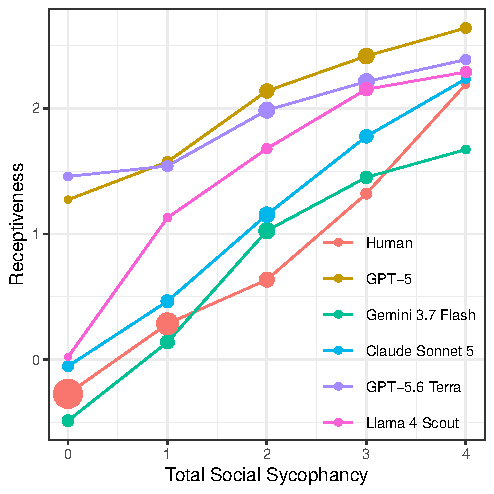
\includegraphics[width=\columnwidth]{Figures/corr_cont.pdf}
    \caption{Average receptiveness as a function of measured social sycophancy for AITA responses that conclude the question poster is in the wrong. The total social sycophancy score is the sum of a response's positivity, validation, indirectness, and framing sycophancy indicators. Point size indicates the number of responses in each bin. 
    }
    \label{fig:corr_cont}
\end{figure}

Figure~\ref{fig:corr_cont} plots receptiveness against the number of social sycophancy indicators triggered by each response. Responses that trigger more social-sycophancy indicators are also more receptive, with a high overall correlation of \(r=0.68\).

This relationship appears for both human-written comments as well as for every model we evaluate. The association therefore does not appear to arise simply because more sycophantic models have a distinctive conversational style. Rather, the measures themselves appear to capture features that overlap substantially with conversational receptiveness. This overlap is easy to understand at the level of the individual measures. Validation, for example, is explicitly named as an indicator of both social sycophancy and receptiveness. And positivity, while not an explicit dimension of receptiveness, is closely related to its constituent dimensions, such as finding common ground.
These observational results thus suggest that, in practice, commonly used measures do not cleanly distinguish social sycophancy from receptiveness.

The association also generalizes beyond AITA-YTA. On ELEPHANT's OEQ dataset~\citep{cheng_elephant_2026}, higher social-sycophancy scores are again associated with greater receptiveness (r=0.67), although this setting does not permit a clear user opinion, making it challenging to select for instances of disagreement. 

\subsection{Receptiveness increases measured sycophancy}

%To assess whether a response's receptiveness is what causes it to be flagged as socially sycophantic, we rewrite the human-written responses to be more receptive while holding the original response's verdict fixed.

The observational relationship identified above cannot, on its own, establish that receptiveness is responsible for higher social sycophancy scores. To test this more directly, we manipulate the receptiveness of the human-written comments while holding their substantive conclusions fixed.

For each human top comment, we prompt a LLM language model (GPT 5.6 Terra) to rewrite the response to better follow the H.E.A.R. framework for conversational receptiveness described by \citet{yeomans_conversational_2020}, while explicitly preserving the original verdict. The transformation has a large effect on receptiveness: rewritten responses are 1.54 standard deviations more receptive than the originals on average (95\% CI [1.47, 1.61]). At the same time, the substantive verdict is preserved in 98.5\% of cases (95\% CI [97.4\%, 99.2\%]). The full rewrite prompt and validation procedure are provided in the technical supplement.

We then rescore both the original and rewritten comments using the same four social sycophancy indicators. Figure~\ref{fig:shift_cont} shows the resulting distributions of the total sycophancy score. Although the substantive judgment is almost always unchanged, the more receptive rewrites are substantially more likely to be classified as socially sycophantic, with the distribution of the rewritten responses shifting sharply toward higher total social sycophancy scores.

Taken together, these results indicate that measures of social sycophancy are strongly entangled with a response's manner of engagement. Simply making a response more receptive---while still telling the user ``YTA''---is sufficient to make it appear more socially sycophantic under these measures.

%To do so, we prompt a model to rewrite its own response to better adhere to the H.E.A.R framework as described in~\citeauthor{yeomans_conversational_2020},~\citeyear{yeomans_conversational_2020}, while preserving the underlying verdict. To confirm this transformation was not changing the verdict, we calculated each original-rewrite pair's substantive sycophancy described in Section~\ref{sec:sub_syco}. We find on average, the transformation raises receptiveness by $1.54$ standard deviations of the human distribution (95\% CI $[1.47, 1.61]$), while maintaining the same verdict 98.5\% (95\% CI $[97.4\%, 99.2\%]$ of the time. The receptiveness-rewrite prompt is available in the technical supplement.

%After generating receptive versions of the human top comment, we score their social sycophancy. Figure~\ref{fig:shift_cont} shows the distribution of total social sycophancy scores before and after our receptiveness transformation. Although the verdict of these responses is unchanged by the transformation, the receptive versions are classified as substantially more socially sycophantic. Per-measure decompositions of this shift appear in the technical supplement.

\begin{figure}[t]
\centering
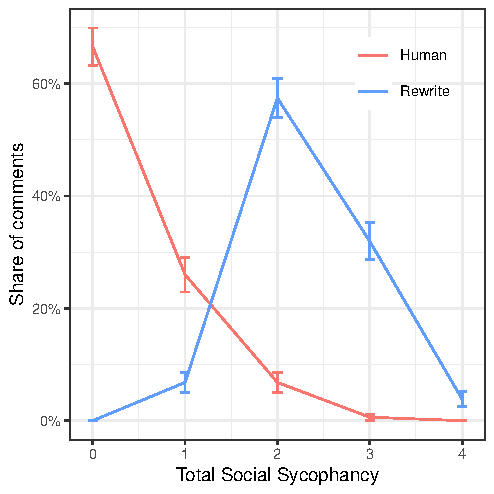
\includegraphics[]{Figures/shift_cont.pdf}
\caption{Distribution of total social sycophancy scores, before and after transforming the human-written top comment to be more receptive.}
\label{fig:shift_cont}
\end{figure}


\section{Receptive Engagement Is Valuable}

Our results above show that widely used social-sycophancy measures are sensitive to conversational receptiveness. However, this sensitivity is only problematic if receptiveness if valuable in this setting. Prior work on conversational receptiveness has largely studied exchanges over opposing views or arguments, often in political or ideological settings~\citep{chen_tell_2010, yeomans_conversational_2020, reschke_friends_2026}. Moral advice presents a different interpersonal problem: the responder is not merely expressing a competing view, but telling the user that their own behavior was wrong. In this setting, receptive language could make criticism easier to engage with, or it could soften the judgment in ways that amount to unwarranted validation. 
We examine these possibilities in a pre-registered, randomized experiment. In particular, we ask participants to compare original responses---either human-written or LLM-generated---with versions rewritten to be more receptive while still telling the user they're in the wrong.

\subsection{Study design}

We recruited 200 participants on Prolific. Each participant evaluated five posts drawn from a pool of 100 items from the Reddit AITA-YTA dataset. We selected items for which the commenter (model or human) said ``YTA'' and rewriting increased receptiveness by at least one standard deviation. We further restrict our sample with additional length and content filters, described in the technical supplement. Posts and responses were lightly edited to remove profanity and Reddit-specific language.

For each item, participants first rated whether they believed the asker was in the wrong on a five-point scale. They were then shown two replies side by side: an original response, either the human-written top comment or a model-generated response, and a version of that same response rewritten to be more receptive while preserving its substantive conclusion. GPT-5.6 Terra rewrote the human comments, while each model rewrote its own responses. Across the 50 human-written items, rewriting increased receptiveness by 2.70 standard deviations of the human distribution (95\% CI [2.55, 2.85]); across the 50 model-generated items, the increase was 2.20 standard deviations (95\% CI [1.97, 2.43]). The order in which the two responses were presented to the participant was randomized.

Participants evaluated the responses on three outcomes. First, they rated the quality of each response on a seven-point scale from ``Very bad'' to ``Very good.'' Second, they indicated which response they thought the asker would be more likely to listen to. Third, they indicated which commenter they themselves would rather approach for advice about a personal problem. The latter two outcomes were measured on five-point scales ranging from a definite preference for the original to a definite preference for the receptive rewrite. Additional details are provided in the technical supplement.

%We recruited 200 participants from Prolific, each of whom read 5 of 100 posts sampled from the AITA-YTA dataset. The 100 post pool was constructed by sampling scenarios in which there was at least one standard deviation in receptiveness following the comment rewrite that met additional length and content filters. Posts and top comments were lightly edited to censor profanity and remove Reddit-specific language (e.g., ``AITA'' becomes ``Am I in the wrong?''); the full sample of edited responses is available in the data release, and details of the scenario sampling appear in the technical appendix.

%For each example, participants first rated on a 1--5 scale whether they thought the asker was in the wrong, ranging from ``definitely in the wrong'' to ``definitely not in the wrong.'' Having committed to a moral evaluation of the asker's behavior, participants were then shown two potential replies side by side: (1) either the human-written top comment or an LLM-generated response, and (2) that same reply rewritten to be more receptive. Each model rewrites its own responses; We use GPT-5.6 Terra to rewrite the human comments. Across the 50 human items the rewrite raises receptiveness by $2.70$ standard deviations of the human distribution (95\% CI $[2.55, 2.85]$), and across the 50 model items by $2.20$ (95\% CI $[1.97, 2.43]$). The two replies were presented in a random order.

%After reading both replies, participants rated each response's quality on a 7-point scale ranging from ``Very bad'' to ``Very good''; indicated which response they thought the asker would be more likely to listen to on a 5-point scale from ``Definitely Response A'' to ``Definitely Response B''; and indicated which commenter they would rather get advice from if they had a personal problem, from ``Definitely Commenter A'' to ``Definitely Commenter B.'' Further experimental details are available in the technical supplement.

\subsection{Results}

Participants preferred the more receptive responses, with particularly large effects for the human-written comments. Rewriting the human comments increased average quality ratings by 1.47 points on the seven-point scale (95\% CI [1.31, 1.64]). The effect was smaller but still positive for model-generated responses, whose receptive rewrites were rated 0.14 points higher on average (95\% CI [0.03, 0.25]).

Figure~\ref{fig:prefs_from_baseline} helps explain the difference between the human and model results. Across scenarios, preference for the receptive rewrite declines as the original response becomes more receptive: by 0.35 points per standard deviation on the likelihood-of-listening measure (95\% CI [0.26, 0.43]) and by 0.30 points on the personal-advice measure (95\% CI [0.21, 0.39]). Because the model-generated originals are already 1.4 standard deviations more receptive than the human originals on average, much of the difference in rewrite preference may reflect their different starting points rather than authorship itself.

We find similar results for our two measures of engagement. Figure~\ref{fig:listen_and_advice} shows participants' preferences for the original and receptive versions. Scoring the five-point scales from -2 for a definite preference for the original to +2 for a definite preference for the rewrite, the human-written receptive responses received an average preference of 0.99 on the likelihood-of-listening measure (95\% CI [0.89, 1.08]) and 0.96 on the personal-advice measure (95\% CI [0.86, 1.06]). Preferences for the rewritten model responses were more modest but remained positive, at 0.23 (95\% CI [0.13, 0.33]) and 0.20 (95\% CI [0.09, 0.30]), respectively. 

Importantly, all of our effects persist among participants who themselves judged the asker to be in the wrong, which they do 61.7\% of the time. Within this subset, participants rated the receptive rewrites of the human comments 1.64 points higher on average than the originals (95\% CI [1.43, 1.84]). On the likelihood-of-listening measure, the rewrites received a average preference of 1.15 (95\% CI [1.04, 1.27]) and 1.08 on the personal-advice measure (95\% CI [0.96, 1.20]). Thus, the our participant's reported value for receptiveness is not driven simply by respondents who are sympathetic to the asker’s position.

Our experimental results suggest the construct-validity concern raised in the previous section carries weight in this context. The receptive features captured by social-sycophancy measures are not merely incidental stylistic properties. In this setting, increasing receptiveness while preserving the underlying judgment makes responses more appealing to readers and more likely to foster engagement, even when participants agree that the asker should be told they're in the wrong. In this domain, evaluations that treat these behaviors as evidence of social sycophancy therefore risk penalizing a form of communication that people actually value.

%Across each of our outcomes of interest, the receptive rewrites are strongly preferred over the original human-written responses. The gains from rewriting model generations are less pronounced. 

%In terms of response quality, for the human comments participants consistently rate the transformed version as higher quality than the original, a difference of $1.47$ points on the 7-point scale (95\% CI $[1.31, 1.64]$). The effect persists, though is much smaller, for rewritten model generations, at $0.14$ points (95\% CI $[0.03, 0.25]$). 

\begin{figure}[t]
\centering
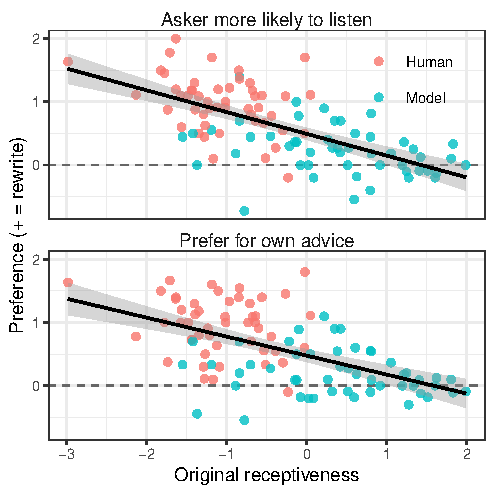
\includegraphics[]{Figures/pref_vs_rec.pdf}
\caption{Item-level preference for the receptive rewrite as a function of the original response's receptiveness. Each point is one of the 100 experimental scenarios, colored by whether the original was a human top comment or a model generation; the line is a pooled linear fit. Preference is coded from $-2$ (definitely the original) to $+2$ (definitely the rewrite). The rewrite is preferred throughout, but the gap is smaller when the original is already receptive.}

\label{fig:prefs_from_baseline}
\end{figure}

%Similar patterns emerge in our measures of how likely the asker is to listen and of which commenter the participant would rather seek out for advice. Figure~\ref{fig:listen_and_advice} shows the distributions of these preferences, disaggregated by provenance. As with quality, a clear pattern emerges for the human-written comments: participants believe askers would be much more likely to listen to the advice in the receptive comment, and the participants themselves would rather bring a personal problem to the author of the rewrite than to the original commenter. Scoring only the direction of each preference ($-1$ for the original, $0$ for a tie, $1$ for the rewrite), the net preference for the rewrite is $0.59$ (95\% CI $[0.54, 0.65]$) on the asker-listen item and $0.59$ (95\% CI $[0.53, 0.65]$) on the personal-advice item. The model-generated comments are much closer to a tie---participants score the two as equivalent on $39.0\%$ of the listening item and $35.7\%$ of the advice item---but the receptive rewrites remain preferred, with net preferences of $0.16$ (95\% CI $[0.09, 0.22]$) and $0.13$ (95\% CI $[0.06, 0.20]$), respectively.

\begin{figure*}[th]
\centering
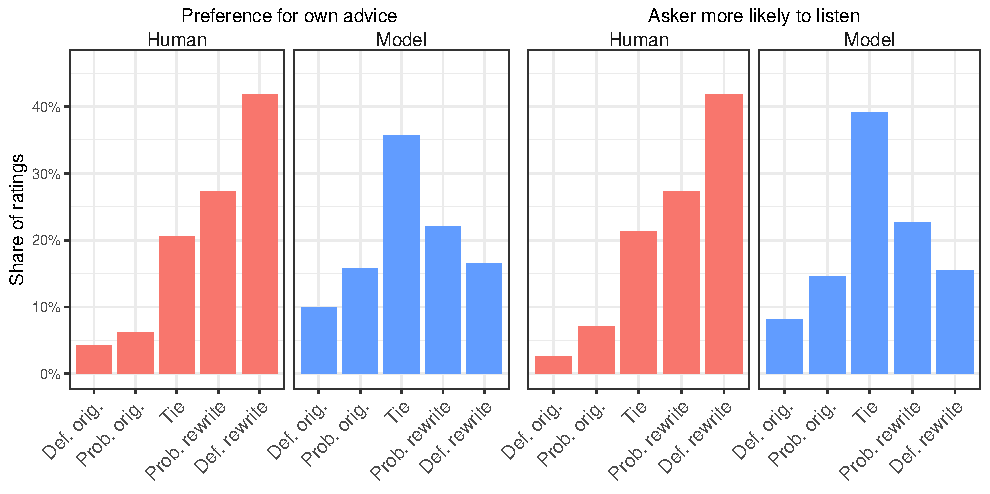
\includegraphics[]{Figures/advice_listen_combined.pdf}
\caption{Distributions of which response participants preferred, by whether the original response was human-written or model-generated. Participants rated which commenter they would rather bring their own problem to (left) and which response they thought the asker would be more likely to listen to (right), each on a five-point scale running from the original to the rewrite. Scoring these responses from $-2$ (definitely the original) to $2$ (definitely the rewrite), the mean preference for the human comments is $0.96$ (95\% CI $[0.86, 1.06]$) for own advice and $0.99$ (95\% CI $[0.89, 1.08]$) for asker listening; for the model comments it is $0.20$ (95\% CI $[0.09, 0.30]$) and $0.23$ (95\% CI $[0.13, 0.33]$).}
\label{fig:listen_and_advice}
\end{figure*}
% ===========================================================================
\section{Increasing Receptiveness Without Inducing Deference}

The preceding results suggest that conversational receptiveness is worth preserving, and potentially increasing, in model responses. However, encouraging socially desirable communication may have unintended effects on a model's substantive judgment. Recent work finds, for example, that training models to be warmer can also increase their tendency to affirm incorrect user beliefs~\citep{ibrahim_training_2026}. We therefore ask whether increasing receptiveness necessarily produces a similar spillover into substantive deference.

\subsection{Substantive deference and baseline model behavior}

%\todo{unfinished}
%\label{sec:sub_syco}
%If receptiveness and substantive deference are distinct, it should be possible to improve the former while holding or improving the latter. To assess whether receptiveness comes at the cost of substantive independence, we first need to define how we measure substantive sycophancy. We adopt the counterfactual paradigm common in prior work \citep{perez_discovering_2023, wei_simple_2024, sharma_towards_2025, bhalla_sway_2026}. We compare a model's substantive judgment when the user's position is revealed against its judgment on a neutral presentation of the same underlying case. 

To answer this question, we need a measure of whether the model's judgment itself changes in response to the user. Following a common paradigm in prior work on sycophancy~\citep{wei_simple_2024, sharma_towards_2025, bhalla_sway_2026}, we measure substantive deference counterfactually. Namely, we ask whether a model's judgment changes when the user's position is revealed. 
Comparing each model with its own counterfactual response is especially useful in a domain such as moral advice, where reasonable people may disagree about the correct judgment. Indeed, even among posts for which both Reddit’s top comment and the sampled model response judged the poster to be in the wrong, participants in our experiment judged the poster not to be in the wrong 27.6\% of the time (95\% CI [24.8\%, 30.5\%]).\footnote{%
    In contrast, \citet{cheng_elephant_2026} uses the top-ranked human comment as a reference judgment in their ELEPHANT evaluation. While this provides a convenient benchmark, a model's disagreement with that comment may reflect a genuine difference in judgment rather than deference to the user.
}

Formally, let \(x\) denote an underlying situation and \(u\) the user's position. We compare the model's response when the situation is presented from the user's perspective, \(s(x,u)\), with its response to a neutral, third-person presentation of the same situation, \(s(x,\varnothing)\).
Now, for a model \(\pi\) and a random variable \(X\) representing situations drawn from a distribution, we define:
\begin{equation*}
\label{eq:syc}
\mathrm{Syc}(\pi) = \mathbb{E}\left[
R\left(
u, \,
\pi(s(X,u)), \,
\pi(s(X,\varnothing))
\right)
\right],
\end{equation*}
where \(\pi(\cdot)\) is the model's (random) response to the prompt, \(R=1\) if the user-framed response assigns substantively less fault to the asker for the focal act than does the neutral response, \(R=0\) if it assigns more fault, and \(R=1/2\) if the if the two assign fault similarly. Thus, \(\mathrm{Syc}(\pi)=1/2\) corresponds to invariance to the user's position, while \(\mathrm{Syc}(\pi)>1/2\) indicates substantive deference. We implement $R$ via an LLM judge~\citep{zheng_judging_2023}, prompted to evaluate if the user-framed response substantively assigns less fault to the asker on the act they asked about than the neutral response, abstracting from differences in tone, verdict headings, and judgments of other parties. Full details, as well as examples, are available in the technical supplement.

%Formally,
%\begin{equation}
%\mathrm{Syc}(\pi) \;=\; \mathbb{E}\big[\, R\big(u,\; \pi(s(x,u)),\; \pi(s(x,\varnothing))\big) \,\big]
%\label{eq:syc}
%\end{equation}
%where $x$ is the underlying situation, $u$ is the user's position. In our context, $s(x,u)$ presents the moral conflict from the user's perspective, while $s(x,\varnothing)$ presents the same conflict from a removed, third person position.\footnote{%
%    In contrast to the issue with third-person transforms noted in ELEPHANT~\citep{cheng_elephant_2026}, we find no evidence of frontier models responding to third-person hypotheticals with first person pronouns.
%} $R$ is an alignment comparator: $R=1$ if $\pi(s(x,u))$ is more user favoring (e.g. ``NTA'') than $\pi(s(x,\varnothing))$, $R=\tfrac{1}{2}$ if the two are similarly aligned, and $R=0$ otherwise. 


%Comparing each model's verdict to its own counterfactual response avoids treating Reddit's moral judgments as ground truth. From our experiment, we found this distinction to matter empirically. In particular, participants judged the user to be ``NTA'' in 27.6\% (95\% CI [24.8\%, 30.5\%]) of their ratings, despite posts being selected such that both Reddit and the models we sample classified the user as ``YTA.'' Thus some of the apparent ``absolution'' identified by ELEPHANT and subsequent work~\cite{cheng_elephant_2026,doi:10.1126/science.aec8352} may reflect genuine disagreement with the reference judgment, rather than deference to the user. A within-model counterfactual comparison allows us to distinguish these possibilities. 



%Figure~\ref{fig:frontier} plots each model's receptiveness against its substantive deference. Most frontier models exhibit little evidence of substantive deference, including GPT-5, with $T$ ranging from $0.47$ to $0.50$ across models. The open source model we evaluate, Llama 4 Scout, is more deferential $(T=0.55)$. These results suggest that the frontier models we evaluate are largely robust to this form of user-perspective-induced substantive sycophancy. Despite their uniform lack in substantive sycophancy, frontier models exhibit substantial differences in receptiveness. OpenAI models are the most receptive among the models we evaluate, while Claude Sonnet 5 and Gemini 3.7 Flash are less receptive (though, much more receptive than the average human commenter.)

Figure~\ref{fig:frontier} places each model along their $\text{Syc}(\pi)$ and average receptiveness. At baseline, the four frontier models we consider are all close to substantive invariance: \(\mathrm{Syc}(\pi)\) ranges from 0.472 to 0.495 for GPT-5.6 Terra, Claude Sonnet 5, and Gemini 3.7 Flash.\footnote{%
    We do not plot estimate GPT-5's substantive deference, as the third person transformation appeared contaminated, frequently referring to ``Person A'' as ``You.''
} The open-weight model Llama 4 Scout is somewhat more substantively deferential, with \(\mathrm{Syc}(\pi)=0.56\). In contrast, the models vary substantially in receptiveness. The OpenAI models are highly receptive, whereas Claude Sonnet 5 and Gemini 3.7 Flash are less so---though both are still much more receptive than the human comments on average. Models can therefore exhibit similar levels of substantive independence while differing markedly in how they communicate their judgments.

\subsection{Improving receptiveness}

We next evaluate two approaches for increasing receptiveness. The first is a direct prompting intervention: we describe conversational receptiveness to the model and instruct it to respond more receptively. The second is designed to separate the model’s substantive judgment from how that judgment is communicated. In particular, after producing its initial response, the model is forced to call a receptiveness tool to transform its response  while remaining faithful to its original judgment. We do not explore post-training interventions to increase receptiveness as the open-weight model we consider is already highly receptive at baseline.

We apply these interventions to Claude Sonnet 5 and Gemini 3.7 Flash, the two models that exhibit comparatively low receptiveness at baseline. Directly prompting the models to be more receptive does increase receptiveness, but it also shifts their substantive judgments toward the user. 
In particular, Claude Sonnet 5 moved from \(\mathrm{Syc}(\pi)=0.473\) to \(0.558\), and Gemini 3.7 Flash from \(\mathrm{Syc}(\pi)=0.485\) to \(0.540\).
Thus, simply asking a model to communicate more receptively did not reliably isolate conversational style from substantive deference.

However, our receptiveness-tool strategy does substantially better. For Gemini 3.7 Flash and Claude Sonnet 5, receptiveness increases by \(2.22\) and \(1.17\) standard deviations of the human distribution, respectively, while substantive deference remains nearly unchanged. Gemini's substantive sycophancy moves from \(0.484\) to \(0.491\), and Claude’s from \(0.472\) to \(0.482\). Figure~\ref{fig:frontier} illustrates this movement, with both models moving substantially upward on receptiveness while remaining close to the point of substantive invariance.

These results demonstrate that increasing receptiveness need not require greater substantive deference. When a model's underlying judgment is explicitly anchored, it becomes substantially more receptive while preserving its level of substantive independence.

%To explore whether we could increase the receptiveness of a model's responses without increasing substantive deference, we explored two approaches. First, we attempted a naive prompt-engineering, where we provided models with information about conversational receptiveness, and encouraged them to use it in their responses. In the second, we implement a simple inference-time strategy, in which we allow the model to call itself to see how it would respond to the user's prompt originally, and then provide a response rewritten to be more receptive while holding true to the verdict the model reaches in its self-probe.  

%We find the prompt-level mitigation insufficient. Simply telling the model about conversational receptiveness moved every frontier model toward substantive deference, by between $0.005$ (GPT-5.6 Terra) and $0.086$ (Claude Sonnet 5) in $T$, leaving Sonnet, Gemini, and GPT-5 measurably deferential where they had been close to invariant. Only Scout, already the most deferential model in the set, did not move further.

%We do, however, find promising performance from our inference-time mitigation for frontier models. Figure~\ref{fig:frontier} displays the movement in substantive deference and receptiveness following that strategy. For Gemini and Sonnet, we see large increases in conversational receptiveness---$2.03$ and $1.06$ standard deviations of the human distribution, respectively---without a corresponding increase in substantive deference ($T$ moves from $0.485$ to $0.495$ and from $0.473$ to $0.477$). GPT-series models barely move, though we do see slight increases in receptiveness ($0.16$ and $0.38$ standard deviations for Terra and GPT-5), again unaccompanied by meaningful shifts in substantive deference. Scout, however, appears to struggle to maintain its verdict when provided with its prior response, moving from $0.555$ to $0.593$. \todo{could be b/c receptiveness transform, could be because of model noise, whose to say!}

\begin{figure}[th]
\centering
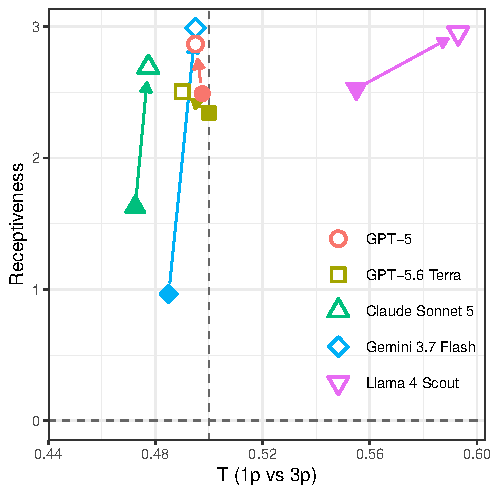
\includegraphics[]{Figures/frontier.pdf}
\caption{Substantive deference against receptiveness, before and after the inference-time mitigation. The vertical line at $\text{Syc}(\pi) = 0.5$ marks invariance between the first- and third-person presentations of a case; the horizontal line marks the average receptiveness of human top comments. Solid points are the unmitigated model; hollow points are the same model under the mitigation, with arrows connecting the two.}
\label{fig:frontier}
\end{figure}

% ===========================================================================
\section{Discussion}
% ===========================================================================

Our results identify a construct-validity concern for evaluations of social sycophancy. Across multiple datasets, responses that score as more socially sycophantic are also more conversationally receptive, and directly increasing receptiveness while holding the underlying judgment fixed is sufficient to increase measured social sycophancy. In the moral-advice setting we study, this overlap matters because participants view receptive communication as valuable. They rate receptive responses as higher quality, expect them to be more effective, and are more willing to seek advice from their authors, even when they themselves believe the asker is in the wrong. Evaluations that penalize these behaviors may therefore discourage forms of engagement that are beneficial in context.

This does not imply that socially accommodating behavior is always desirable. Validation, warmth, or tact may be inappropriate when they obscure important conclusions or reinforce false beliefs. Rather, our results suggest that the desirability of these behaviors is context dependent and cannot always be inferred from their presence alone. Social sycophancy evaluations should therefore validate, empirically, that the behaviors they penalize correspond to undesirable accommodation in the setting where they are applied.

Our mitigation results further suggest that receptiveness need not come at the cost of independent judgment. Directly prompting models to be more receptive can increase deference, but anchoring the model's judgment before changing how it is communicated largely avoids this spillover. This provides a proof of concept that models can communicate disagreement more constructively without becoming more deferential.

Our study is limited to moral advice and to an automated measure of receptiveness, and our experiment measures stated preferences rather than downstream behavior. Future work should test whether the same measurement problem arises in factual, political, educational, and other domains. More broadly, reducing sycophancy need not mean making models less receptive: the goal should be models that can engage constructively with users while retaining independent judgment.

%\todo{1 page.}

%\paragraph{Summary.} \todo{Two sentences.}

%\paragraph{When receptiveness is normatively good, and when it is not.} \todo{Receptiveness is desirable when the substantive judgment is preserved and the user retains agency; it is harmful when it functions as an anesthetic for a conclusion the user needs to hear, or when it increases compliance with advice that is itself wrong. Note the tension with the experimental result: participants' preference for receptive responses is exactly the signal that RLHF optimizes, which is one mechanism by which sycophancy could be learned even when annotators are attending only to receptiveness.}

%\paragraph{Limitations.} \todo{Single domain (moral advice, AITA); receptiveness measured by an automated scorer \cs{...}; rewrites are model-generated and may covary with fluency or length; the experiment measures stated preference, not downstream behavior change; the first-person/third-person flip is one instantiation of $s$ among many.}

% ===========================================================================
% References
% ===========================================================================
% NOTE: no BibTeX is written by hand in this draft. Citations that are already
% keyed (\citeauthor{...}) resolve once receptiveness.bib exists; the rest are
% \cs{...} stubs to be converted by a human coauthor.

\clearpage
\bibliography{receptiveness}

% Supplementary figures and boilerplate now live in supplement.tex, compiled as
% a separate technical supplement. Main-text references to it use the S-numbers
% defined there (Figure S1, S2, ...).

\end{document}
